\documentclass[a4paper,10pt]{article}
\usepackage[utf8]{inputenc}
\setcounter{secnumdepth}{5}
\setcounter{tocdepth}{5}
%opening
\title{Clustering para la clasificación de ítems representados por la web semántica}
\author{Guido Zuccarelli}
\usepackage{graphicx}
\begin{document}

\maketitle

\begin{abstract}
Este trabajo mostrará la metodología, implementación y resultados de un caso en el cuál, partiendo de un dataset que contiene datos 
extraídos de la web semántica, se realizó un proceso de clasificación utilizando algún algoritmo de clustering de minería de datos 
para lograr que los ítems del dataset que representan productos, posean un atributo label, que indique de qué tipo de producto se 
trata. \\
Este proceso se convierte en un paso de integración en un trabajo de desarrollo de una aplicación que utilice datos de la web semántica, 
ya que se agruparán ítems mediante los clusters a los cuales fueron asignados.
\end{abstract}
\newpage
\tableofcontents

\section{Introducción}

\subsection{Dataset semántico}

Un dataset semántico está compuesto por un conjunto de documentos extraídos de la web, que a su vez poseen un conjunto de recursos
clasificados según su representación en el mundo real. Estos recursos pueden representar objetos tanto físicos como abstractos como por ejemplo: Autos, Libros, Ideas, 
Servicios, Plantas, etc.
Este dataset se almacena en una base de datos, la cuál tiene una forma especial para acceder a los datos. Mediante consultas SPARQL, o 
mediante la utilización de frameworks como Jena.
Dichos recursos pueden relacionarse entre sí mediante lo que se denomina propiedades, como por ejemplo un Recurso libro, puede estar 
relacionado, con un recurso Review, mediante la propiedad ``review''. De manera que un documento semántico puede representarse en forma de grafo, 
donde cada nodo es un recurso, y cada arista es una propiedad.


\subsection{Ontologías}

Es la representación abstracta de la taxonomía de los ítems, bajo la cual se encuentran definidos todos los recursos de la web semántica.
Está formada por un conjunto de clases y relaciones entre ellas, de manera que se puede definir un ítem como individuo de una o más clases 
de cualquier ontología. Cada clase y relación está definida bajo un namespace que la identifica unívocamente.
Existen, muchas distintas ontologías en la web que modelan diferentes dominios. 
La clase de un ítem, también puede ser llamada tipo. Y funciona de manera similar a la programación orientada a objetos. 

\subsection{Item}

Llamaré ítem, a los recursos de clase ``Producto'' del dataset que estén relacionados con al menos un recurso Review. Estos recursos pueden reprensentar 
múltiples tipos de producto, como por ejemplo: Películas, Ropa, Hardware, etc, los cuales se intentará identificar mediante la clusterización.
Estos ítems tendrán información representativa, establecida por propiedades y otros recursos.

\subsection{Review}

Es un recurso de clase ``Review'' que se relaciona con un recurso Ítem mediante la propiedad ``review''. Representa la evaluación de dicho ítem 
de parte de un usuario y está compuesto principalmente por un puntaje numérico y una evaluación textual. \\

\subsection{K-Medias}

Es un algoritmo de agrupamiento que utiliza aprendizaje no supervisado para resolver una clusterización, en K número de clusters (prefijado).\\
Utiliza K puntos aleatoria o arbitrariamente dispersos en el mapa, que serán llamados centroides. El algoritmo entonces, en varias etapas (también prefijadas) 
intenta aproximar esos puntos a los clusters, asignándoles los elementos más cercanos.
Se pueden utilizar varias medidas de distancias, entre las que se encuentran la distancia euclidiana cuadrada, o la distancia Itakura Saito.

\subsection{Modelo de clustering}

Es el resultado de aplicar un algoritmo de clustering, que esta compuesto por la ubicación de sus centroides. Dichos modelos pueden ser utilizados 
agrupar los datos, simplemente con asignarlos al centroide más cercano. 

\subsection{TF-IDF}

Es una de las más populares medidas que se usa para representar el valor numérico de la información de un documento de texto estructurado en una lista de palabras en consideración a un conjunto de documentos.
Esta medida pondera cada palabra de un texto, otorgándole un puntaje que depende de cuántas veces dicha palabra se encuentra en un documento, y cuán frecuente 
es esa palabra en otros documentos.

\subsection{Silohouette Coefficient}

Es una medida que le otorga un valor numérico entre -1 y 1 a la correctitud de la ubicación de un ítem en un cluster, para luego, otorgar un mismo 
rango de puntaje a un modelo de clustering, promediando los valores del conjunto de ítems aplicados a dicho modelo.\\
Esta medida considera la distancia del ítem con respecto al conjunto de ítems de su mismo cluster, y luego al resto de los ítems. De manera que,
cuanto menor distancia haya con respecto a los de su mismo cluster y mayor distancia con respecto a ítems de clusters foráneos, mejor puntaje obtendrá.

\subsection{SPARQL}

Es un lenguaje de consultas que se utiliza para acceder y modificar información de un dataset semántico. Para esto se utiliza un motor específico que depende 
de cómo esté almacenado el dataset semántico. Suele ser bastante flexible, pero no admite demasiada manipulación de los datos resultantes. 
Se puede combinar la información que retorna pero suele ser con queries muy complejas que además demandan mucho timepo de ejecución.

\section{Problema planteado}

Se dispone de un dataset semántico que contiene 16661 recursos de tipo Producto (clase definida bajo la ontología schema.org). 
Dicho tipo, no es la mejor representación que puede obtener el ítem, dado que un Producto es un tipo muy abarcativo y puede representar 
también, múltiples otros tipos de clase. Como por ejemplo, un producto puede también ser un utensillo, o música. \\
\\
La ontología schema, define una taxonomía de 946 clases, y esos 16661 ítems, deberían estar mejor distribuidos bajo la mismo, que agrupados 
todos juntos en la clase Producto. \\
Para esto se dispone de información representativa de cada ítem, que ayudará a describir al mismo e intentar establecer un nuevo tipo que 
defina al mismo.

\section{Objetivos}

En base al caso de estudio planteado en la sección  anterior, mediante la implementación de algún algoritmo de clustering de minería de datos 
se definen los siguientes objetivos:

\begin{enumerate}

 \item Agrupar los ítems, que representan el mismo dominio de información. Esto es, reconocer los recursos que tienen el mismo tipo,
 como por ejemplo, agrupar todos los ítems de tipo película
 
 \item Etiquetar aquellos grupos encontrados de acuerdo al tipo de información que representan.
 
 \item Reconocer a qué clase de la ontología schema.org pertenecen aquellos grupos encontrados, si es que existe alguna.
 
 \item Verificar la performance de los clusterings realizados en base a métricas ya definidas.
 
 \item Evaluar las distintas posibles configuraciones del algoritmo de clustering elegido.
 
 \item Intentar establecer una relación entre la performance obtenida para un agrupamiento encontrado, y el éxito obtenido en corresponder 
 los grupos con clases de la taxonomía definida por schema.org
 
\end{enumerate}


\section{Estrategia}

\subsection{Preparación de los datos}

\subsubsection{Selección de los datos}
Dado que se parte de un dataset extremadamente grande, el primer paso es determinar qué recursos se van a seleccionar y qué información 
de los mismos se utilizarán.\\
\\
Las propiedades que relacionan los ítems con otros recursos que se elegirán, tienen que definir información representativa del ítem. 
Por ejemplo una propiedad irrelevante para el caso podría ser itemCondition (que describe si el producto es nuevo o usado). 
En cambio una muy relevante sería su descripción. 
Otro aspecto a tener en cuenta es el grado de abarcatividad de la propiedad en la población, dado que una propiedad puede ser muy descriptiva, pero sólo estar 
presente en un individuo de la misma.\\
\\
En base a los criterios descriptos, las propiedades elegidas fueron:\\\\
Nombre (del producto)\\
Descripción (del producto)\\
Nombre (del review del producto) \\
ReviewBody (del review del producto) \\
\\
La información elegida entonces, se utilizará como representación de un ítem, para lo que deberá conformar entonces una bolsa de palabras.\\
También cada ítem está identificado por un id único en el dataset.\\ 
Los datos resultantes deberán tener una estructura organizada en un par de valores para cada ítem, donde el primer valor es el ID del mismo
y el segundo es el conjunto de palabras, proveniente de los valores de las propiedades seleccionadas, separadas por espacio.\\

\subsubsection{Obtención de los datos}
Una vez determinada qué información se requiere, es necesario realizar algunos procedimientos para obtenerla de manera correcta.
Existen algunas situaciones que pueden presentar dificultades para realizar el mismo:\\
\begin{itemize}
 \item Un ítem puede relacionarse con más de un recurso bajo una misma propiedad. Por ejemplo, un ítem puede tener la propiedad nombre dos veces, para poner dos nombres distintos.
 \item Un ítem puede no utilizar una o más de las propiedades escogidas.
 \item Los ítems contienen generalmente más de un review.
 \item Los reviews de los ítems se pueden obtener por dos propiedades distintas.
 \item Los valores de las propiedades pueden contener secuencias de caracteres como \verb|\t o \n| que afectarán la estructura del documento resultante.
\end{itemize}

Una buena forma de obtener la información es a travez de consultas sparql. Ya que proporciona un acceso rápido y eficiente a los datos.
Pero debido a las posibles circunstancias planteadas en el punto anterior, esta estrategia no será suficiente. Se requerirá de un algoritmo en Java
para organizar los datos.\\
Para lograr obtener un documento con la estructura planteada anteriormente, se realizaron los siguientes pasos.
\begin{description}
  \item[First] Primero una consulta sparql que obtenga todos los pares de valores \verb|ID - {valor de la propiedad}|. 
  \item[Second] Luego contando con una estructura de HashMap de java, donde la clave es el ID del ítem y el valor es un ArrayList 
  de Strings, almacenar el valor de la propiedad en un elemento del ArrayList de ese ítem. De manera que al final se obtenga por ítem un ArrayList con cada valor de cada propiedad.
  \item[Third] Una vez confeccionado el HashMap, suprimir todos los posibles valores de \verb|\t o \n| que puedan generar problemas
  \item[Fourth] Por último se puede recorrer el HashMap e imprimir en un archivo, cada ID de ítem, seguido por los elementos de su ArrayList separados por espacio. 
\end{description}

\subsection{Planificación de la estrategia}

\subsubsection{Selección de algoritmo}
En este punto, se deberá escoger alguno de los algortimos de clustering posibles para implementar y así cumplir los objetivos planteados. \\
Las opciones son muchas, y varían en distintos tipos:\\\\
Algoritmos basados en conectividad (que pueden ser aglomerativos y divisivos)\\
Algoritmos basados en centroides\\
Algoritmos basados en modelos de distribución\\
Algoritmos basados en densidad\\
\\
El algoritmo escogido fue el k-medias, por su relación entre simplicidad y eficiencia. 

\subsubsection{Modelado de los datos}

El algoritmo k-medias requiere manejar un conjunto de datos ponderables para su ejecución, lo que hace que una bolsa de palabras por cada ítem, 
sea insuficiente para su implementación.\\
Es necesario entonces definir una estrategia de modelado de datos que transforme el documento actual con una estructura en forma de bolsa de palabras 
a un modelo que le dé determinado peso a la representación de los ítems.\\
La técnica más comunmente usada en estos casos es la representación en forma de un vector de palabras, donde cada fila representa a un ítem, y 
cada columna representa a determinada palabra, de manera que para N ítems y M palabras, se tienen un total de NxM celdas. Y el valor de cada celda es 
determinado por el algoritmo TF-IDF.
Esto da una representación ponderada de cada ítem.

\subsubsection{Implementación}

Tanto el algoritmo TD-IDF como K-medias son ampliamente utilizados y se encuentran disponibles en múltiples herramientas.\\
Por lo que no es necesario codificar cada uno de ellos, sino que se puede utilizar algunad e estas herramientas.\\
En este caso se optó por la utilización de la herramienta Rapidminer. Que dispone de todos los algoritmos necesarios para realizar 
la implementación.\\
Luego de importar el dataset con la bolsa de palabras los operadores utilizados en rapidminer fueron:\\
\begin{description}
  \item[1 Retrieve] Que selecciona el documento y lo pone a disposición de los operadores. 
  \item[2 Process document from data] Este operador recibe un dataset y lo transforma en un documento. El formato de este documento resultante 
  es configurado en el operador. Por nuestra estrategia decidida, en el campo vector creation se seleccionó TF-IDF luego de haber tildado la casilla ``create word vector''.
  \item[2.1 Tokenize] Dentro del mismo operador se realizo primero un paso de tokenizar (que divide el documento en una secuencia de tokens, donde cada token representaría una palabra).
  \item[2.2 Transform Cases] El siguiente operador es el que lleva todas las palabras a minúscula.
  \item[2.3 Stemming] Y luego se utiliza el operador con snowball que analiza secuencias de palabras con el objetivo de adecuarlas a un idioma. 
  \item[3 Clustering] Una vez procesado el documento, se lo envía al operador de k-medias. Donde se puede configurar el K (la cantidad de centroides, que deriva en la cantidad de grupos creados) \ldots
\end{description}

En cuanto a la configuración de los modelos, se utilizó como valores de K el conjunto de \verb|{9,10,12,13,17,20,25,30}| por lo que la implementación, 
se ejecutó 8 veces, obteniendo así, 8 modelos de clustering distintos para el mismo conjunto de ítems.

\subsection{Análisis de los resultados}

Este punto es el que determina cómo se llevarán a cabo los objetivos. Y se divide en dos formas de llevarlo a cabo\\
Índice de eficacia: Realizado automáticamente por un algoritmo.\\
Análisis experto: Los resultados del clustering son examinados manualmente para determinar qué tan bien funcionó el clustering.\\

\subsubsection{Índice de eficacia}

Se utiliza alguna medida de validación del clustering, generada por un algoritmo a elección.\\
Existen varios algoritmos, entre los que sen encuentran: \\\\
Davies–Bouldin index\\
Dunn index\\
Silhouette coefficient\\
\\
Se optó por el Silhouette coefficient en base a que es la opción que mejor funciona con un clustering realizado por el algoritmo k-medias 
dado que ayuda a determinar cuál es el número óptimo de clusters configurable del algoritmo.\\
\\
Si bien este algoritmo se encuentra disponible como operador en rapidminer, su elevado orden de ejecución (que llegaría a $$N.M^{2}$$  
siendo N la cantidad de palabras del dataset, y M la cantidad de ítems) sumado a la gran cantidad de datos con los que se trabajan,
hacen que el algoritmo no escale y demore una extremadamente grande cantidad de tiempo. \\
Se codificó entonces, una versión de este algoritmo que utilice programación dinámica, y multithreading para hacerlo ejecutable en un 
razonable período de tiempo por la pc.\\

\subsubsection{Análisis experto}

Consiste en visualizar manualmente una muestra de los resultados, para así poder determinar exactamente cada ítem a qué tipo de producto 
pertenecía, y compararlo con el resto de los ítems de la muestra de su mismo cluster.\\
\\
Una observación de este tipo permitirá:\\
\begin{enumerate}
 \item Identificar a qué tipo de producto pertenecen la mayoría de los ítems contenidos en él. Si es que se consigue una marginal mayoría.\\
 \item Evaluar subjetiva y objetivamente qué tan bien funcionó cada modelo de cluster obtenido. Para poder también relacionarlo con los resultados 
del índice silhouette.
 \item En base al tipo de producto identificado en cada cluster, encontrar una clase en la ontología de schema que lo represente.
\end{enumerate}

El tamaño de la muestra debería estar acotado por la cantidad mínima necesaria de individuos de un cluster necesarios para que conformen 
una muestra representativa, y la cantidad máxima de ítems que humanamente se pueden analizar sin que esta sea una tarea exageradamente larga.\\
\\
Considerando 2500, como la cantidad de ítems adecuada para observar humanamente y hacer de ésta una tarea razonable, se distribuirán, a travez de 
cada cluster de cada modelo de la siguiente manera:\\
$$v_{ij} = 10+\frac{c_{ij}}{100} $$\\
Siendo v = cantidad de ítems analizados para el cluster i del modelo j. Y c la cantidad total de ítems del cluster i del modelo j.\\
Esto da un total de 2558 observaciones.

\subsection{Clasificación}

Por último, una vez obtenidos los resultados, y pudiendo determinar cuál modelo de clustering fue el más adecuado, se puede proceder a 
clasificar los ítems según la ontología schema.org.

Para ello sólo se requiere correr un algoritmo de Java usando la librería de jena, que recorra todos los ítems a los cuales se les pudo 
asignar una clase, y utilizarla junto con la propiedad type.


\section{Resultados}

El proceso de selección de datos arrojó 16661 ítems con sus respectivas bolsas de palabras, que luego pasaron por un procesamiento de texto 
en rapidminer para crear un vector de palabras de TF-IDF.\\
Dicho vector estaba quedó conformado por una matriz de 16661 filas, representando a cada ítem y 49098 columnas, una por cada palabra encontrada 
en almenos un ítem.\\
En base a ese vector, se ejecutaron todos los algoritmos de clustering de distintas configuraciones para el k-medias, utilizando valores de K de 9,10,11,13,17,20,25 y 30. 
También utilizando divergencia de Bregman y como medida de distancia la distancia euclideana cuadrada.\\
El tiempo de ejecución para dichos algoritmos aumentaba, a medida que aumentaba la cantidad de centroides configurados, partiendo desde 10 horas para 
el más corto y 36 horas para el más largo.\\
\\
Una vez concluidos exitosamente todos los algoritmos se procedió a ejecutar el algoritmo de cálculo de silhouette index.\\
Puede observarse en la imagen, que existe una tendencia a mejorar la performance del modelo a medida que el número de centroides 
(K) aumenta. Lo que implica que se debería seguir aumentando dicha configuración, según el índice.


Luego el proceso de análisis manual, dio un panorama mucho más revelador, que el índice.\\
Sobretodo porque se pudieron evaluar aspectos mucho más importantes en consideración a la finalidad de haber realizado el clustering.\\
En Figure 1: Performances por cantidad de centroides se disponen de los resultados de los análisis de cada modelo.\\
\\
Se debe tener en cuenta qué, Cluster es simplemente el número identificador del cluster, Población se refiere a la cantidad de ítems 
dentro del cluster, Tipo es el tipo que humanamente le fue otorgado al cluster (teniendo en considerando que fue necesario realizar una 
abstracción adecuada, por ejemplo muchos clusters que contenían Alfombras para auto, fueron etiquetados como accesorios para Auto), Efectivos 
es la cantidad de ítems dentro del cluster que pertenecían a ese tipo (Observar que un cluster puede contener ítems de múltiples tipos, pero el tipo 
etiquetado al claster representa a la mayoría), y utilidad significa si dicho tipo esta contenido en la ontología de schema.\\
\\
Modelo K9\\
\begin{tabular}{| c | c | c | c | c |}\hline
Cluster & Población & Tipo & Efectivos & Útiles\\\hline
0 & 2240 & Accesorios auto & 2240 & No\\
1 & 601 & Comida & 601 & No\\
2 & 2491 & Vestidos & 2491 & No\\
3 & 963 & Música & 963 & Sí\\
4 & 399 & Accesorios auto & 399 & No\\
5 & 512 & Cuchillos & 512 & No\\
6 & 1714 & Autos & 1714 & Sí\\
7 & 5031 & Libros & 1710 & Sí\\
8 & 2710 & Películas & 1978 & Sí\\\hline
\end{tabular}
\\
\\
Modelo K10\\
\begin{tabular}{| c | c | c | c | c |}\hline
Cluster & Población & Tipo & Efectivos & Útiles\\\hline
0 & 2491 & Vestidos & 2491 & No\\
1 & 536 & Accesorios auto & 536 & No\\
2 & 877 & Accesorios auto & 877 & No\\
3 & 513 & Cuchillos & 513 & No\\
4 & 601 & Comida & 601 & No\\
5 & 945 & Accesorios auto & 945 & No\\
6 & 6191 & Libros & 3590 & Sí\\
7 & 238 & Accesorios auto & 238 & No\\
8 & 2552 & Películas & 1709 & Sí\\
9 & 1717 & Autos & 1717 & Sí\\\hline
\end{tabular}
\\
\\
Modelo K12\\
\begin{tabular}{| c | c | c | c | c |}\hline
Cluster & Población & Tipo & Efectivos & Útiles\\\hline
0 & 609 & Accesorios auto & 609 & No\\
1 & 1423 & Accesorios auto & 1423 & No\\
2 & 1641 & Libros & 1641 & Sí\\
3 & 2702 & Películas & 2242 & Sí\\
4 & 3499 & Películas & 699 & Sí\\
5 & 1885 & Vestidos & 1885 & No\\
6 & 1699 & Autos & 1699 & Sí\\
7 & 601 & Comida & 601 & Sí\\
8 & 499 & Cuchillos & 499 & No\\
9 & 968 & Música & 968 & Sí\\
10 & 658 & Vestidos & 658 & No\\
11 & 477 & Accesorios auto & 477 & No\\\hline
\end{tabular}
\\
\\
Modelo K13\\
\begin{tabular}{| c | c | c | c | c |}\hline
Cluster & Población & Tipo & Efectivos & Útiles\\\hline
0 & 601 & Comida & 601 & No\\
1 & 1462 & Películas & 1462 & Sí\\
2 & 1717 & Autos & 1717 & Sí\\
3 & 513 & Cuchillos & 513 & No\\
4 & 2345 & Accesorios auto & 1336 & No\\
5 & 3801 & Libros & 1634 & Sí\\
6 & 357 & Accesorios auto & 357 & No\\
7 & 876 & Accesorios auto & 876 & No\\
8 & 2492 & Vestidos & 2492 & No\\
9 & 613 & Accesorios auto & 613 & No\\
10 & 238 & Accesorios auto & 238 & No\\
11 & 944 & Música & 944 & Sí\\
12 & 702 & Series & 702 & Sí\\\hline
\end{tabular}\\
\\
Modelo K17\\
\begin{tabular}{| c | c | c | c | c |}\hline
Cluster & Población & Tipo & Efectivos & Útiles\\\hline
0 & 1701 & Autos & 1701 & Sí\\
1 & 216 & Accesorios auto & 216 & No\\
2 & 896 & Música & 896 & Sí\\
3 & 434 & Cuchillos & 434 & No\\
4 & 585 & Accesorios auto & 585 & No\\
5 & 229 & Accesorios auto & 229 & No\\
6 & 240 & Hardware & 120 & Sí\\
7 & 239 & Accesorios auto & 239 & No\\
8 & 1216 & Películas & 1216 & Sí\\
9 & 1899 & Libros & 1709 & Sí\\
10 & 601 & Comida & 601 & No\\
11 & 887 & Accesorios auto & 887 & No\\
12 & 2465 & Vestidos & 2465 & No\\
13 & 184 & Cuchillos & 132 & No\\
14 & 600 & Accesorios auto & 600 & No\\
15 & 648 & Series & 648 & Sí\\
16 & 3621 & Películas & 832 & Sí\\\hline
\end{tabular}\\
\\
Modelo K20\\
\begin{tabular}{| c | c | c | c | c |}\hline
Cluster & Población & Tipo & Efectivos & Útiles\\\hline
0 & 465 & Accesorios auto & 246 & No\\
1 & 80 & Accesorios auto & 80 & No\\
2 & 3874 & Películas & 1045 & Sí\\
3 & 1629 & Libros & 1629 & Sí\\
4 & 2480 & Vestidos & 2480 & No\\
5 & 91 & Accesorios auto & 91 & No\\
6 & 238 & Accesorios auto & 238 & No\\
7 & 802 & Accesorios auto & 802 & No\\
8 & 601 & Comida & 601 & No\\
9 & 295 & Accesorios auto & 295 & No\\
10 & 396 & Accesorios auto & 396 & No\\
11 & 280 & Cuchillos & 280 & No\\
12 & 1282 & Películas & 1282 & Sí\\
13 & 311 & Videojeugos & 311 & Sí\\
14 & 47 & Autos & 47 & Sí\\
15 & 216 & Accesorios auto & 216 & No\\
16 & 675 & Accesorios auto & 675 & No\\
17 & 306 & Cuchillos & 306 & No\\
18 & 921 & Música & 921 & Sí\\
19 & 1672 & Autos & 1672 & Sí\\\hline
\end{tabular}\\
\\
Modelo K25\\
\begin{tabular}{| c | c | c | c | c |}\hline
Cluster & Población & Tipo & Efectivos & Útiles\\\hline
0 & 496 & Cuchillos & 496 & No\\
1 & 117 & Accesorios auto & 94 & No\\
2 & 884 & Música & 884 & Sí\\
3 & 167 & Accesorios auto & 167 & No\\
4 & 599 & Accesorios auto & 599 & No\\
5 & 352 & Series & 352 & Sí\\
6 & 225 & Accesorios auto & 225 & No\\
7 & 1710 & Autos & 1710 & Sí\\
8 & 2708 & Películas & 1354 & Sí\\
9 & 372 & Vestidos & 372 & No\\
10 & 1085 & Vestidos & 1085 & No\\
11 & 393 & Accesorios auto & 393 & No\\
12 & 655 & Accesorios auto & 655 & No\\
13 & 214 & Accesorios auto & 214 & No\\
14 & 480 & Series & 480 & Sí\\
15 & 80 & Accesorios auto & 80 & No\\
16 & 307 & Videojeugos & 307 & No\\
17 & 2213 & Libros & 1881 & Sí\\
18 & 135 & Accesorios auto & 108 & No\\
19 & 293 & Accesorios auto & 293 & No\\
20 & 1074 & Vestidos & 1074 & No\\
21 & 601 & Comida & 601 & No\\
22 & 1050 & Películas & 1050 & Sí\\
23 & 70 & Libros & 31 & Sí\\
24 & 381 & Accesorios auto & 381 & No\\\hline
\end{tabular}\\
\\
Modelo K30\\
\begin{tabular}{| c | c | c | c | c |}\hline
Cluster & Población & Tipo & Efectivos & Útiles\\\hline
0 & 443 & Música & 443 & Sí\\
1 & 1101 & Libros & 1101 & Sí\\
2 & 186 & Accesorios auto & 186 & No\\
3 & 295 & Accesorios auto & 295 & No\\
4 & 484 & Cuchillos & 484 & No\\
5 & 691 & Vestidos & 691 & No\\
6 & 91 & Accesorios auto & 91 & No\\
7 & 237 & Accesorios auto & 237 & No\\
8 & 1595 & Accesorios auto & 669 & No\\
9 & 857 & Vestidos & 857 & No\\
10 & 183 & Accesorios auto & 183 & No\\
11 & 601 & Comida & 601 & No\\
12 & 382 & Accesorios auto & 382 & No\\
13 & 860 & Películas & 860 & Sí\\
14 & 641 & Vestidos & 641 & No\\
15 & 590 & Libros & 590 & Sí\\
16 & 644 & Series & 644 & Sí\\
17 & 230 & Accesorios auto & 230 & No\\
18 & 80 & Accesorios auto & 80 & No\\
19 & 210 & Hardware & 138 & Sí\\
20 & 643 & Autos & 643 & Sí\\
21 & 477 & Accesorios auto & 477 & No\\
22 & 1740 & Películas & 1531 & Sí\\
23 & 1123 & Autos & 1123 & Sí\\
24 & 245 & Accesorios auto & 245 & No\\
25 & 352 & Vestidos & 352 & No\\
26 & 307 & Videojuegos & 282 & Sí\\
27 & 117 & Accesorios auto & 84 & No\\
28 & 774 & Hardware & 774 & Sí\\
29 & 482 & Música & 482 & Sí\\\hline
\end{tabular}
\\
\\
Evaluando entonces el conjunto de clusters de cada model, se puede obtener la siguiente tabla comparativa:\\
\begin{tabular}{| c | c | c | c | c |}\hline
Modelo & \%Etiquetas & \%etiquetas correctas & \%Efectividad & \%Redundancia\\ \hline
9 & 62 & 38 & 75 & 11\\
10 & 62 & 42 & 79 & 30\\
12 & 66 & 47 & 80 & 33\\
13 & 51 & 38 & 80 & 30\\
17 & 61 & 42 & 81 & 41\\
20 & 58 & 41 & 81 & 55\\
25 & 56 & 46 & 89 & 60\\
30 & 53 & 51 & 92 & 63\\ \hline
\end{tabular}

Donde, Modelo, es la cantidad de centroides del modelo, \%Etiquetas es el porcentaje de ítems etiquetados, \%etiquetas correctas es el porcentaje 
de ítems corréctamente etiquedatos, \%Efectividad es el porcentaje de ítems que fueron correctamente agrupados en los clusters. Y \%Redundancia 
es el porcentaje de clústers representando el mismo tipo.\\
\\
Se puede apreciar en Figure 2:Estadísticas por cantidad de centroides el gráfico estadístico obtenido en la última tabla.\\
Y también como disminuye el porcentaje de error en el etiquetado al aumentar la cantidad de centroides e nFigure 3: \% de etiquetas incorrectas por modelo
\begin{figure}
  \centering
    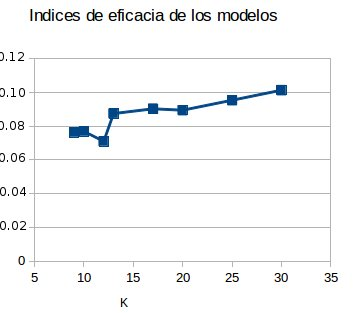
\includegraphics[width=0.7\textwidth]{chart1}
  \caption{Performances por cantidad de centroides}
  \label{fig:ejemplo}
\end{figure}
\begin{figure}
  \centering
    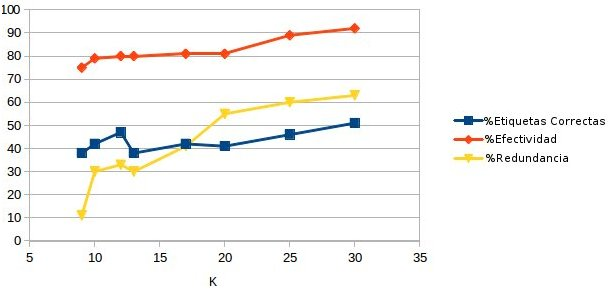
\includegraphics[width=0.7\textwidth]{chart2}
  \caption{Estadísticas por cantidad de centroides}
  \label{fig:ejemplo}
\end{figure}
\begin{figure}
  \centering
    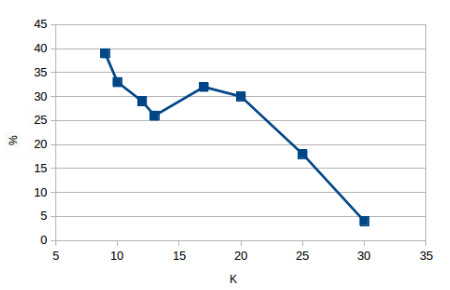
\includegraphics[width=0.7\textwidth]{char3}
  \caption{\% de etiquetas incorrectas por modelo}
  \label{fig:ejemplo}
\end{figure}
\\
\\
Dado que la necesidad de realizar un clustering está dada por la cantidad de ítems correctamente etiquetables bajo la ontología de schema, 
y no por nigún otro parámetro de evaluación, queda entonces decidido por una diferencia notoria el modelo resultanto por el algoritmo de k-medias 
con 30 centroides.


\section{Conclusiones}

En lineas generales los resultados obtenidos fueron muy satisfactorios, se pudieron clasificar el 53\% de los productos con tan solo un 
4\% de margen de error aproximadamente. \\
\\
Hay un marcado progreso en cuanto a la eficiencia de los los modelos de clustering a medida que la cantidad de centroides aumenta. Tanto 
considerando el análisis algorítmico como el análisis experto. También considerando la utilidad del modelo resultante para lograr llevar a cabo el objetivo
de etiquetar dichos ítems, sumado a la disminución de etiquetas incorrectas.\\
Esta situación tiene fundamento en que al ser textos redactados por distintos usuarios la fuente de información con la que se trabaja, provoca que 
los individuos (ítems) estén muy dispersos entre sí. Esto parece provocar que a mayor división entre ellos, mejores resultados se reflejan, considerando los 
parámetros mencionados. De manera que si se utiliza un número mayor o igual de clusters que de ítems, quedando así un ítem por cluster, 
el resultado tanto del índice silouhette como de la efectividad de los clusters sería perfecto.\\
Sin embargo, aumentar considerablemente el número de centroides llevaría a claros problemas, como la cantidad de esfuerzo humano que se requeriría 
para analizar los clusters, o el tiempo de ejecución de los algoritmos. Que es justamente lo que se quiere reducir al utilizar clustering.\\
Por lo tanto el criterio de selección de la cantidad de centroides, debería hacerse considerando la relación entre la mejora que se podría obtener 
aumentando los centroides como la cantidad de esfuerzo horas hombres disponibles.\\


\end{document}
